\documentclass[a4paper, 12pt]{report}
\usepackage[utf8]{inputenc}
\usepackage[T1]{fontenc}

\usepackage{xcolor}
\usepackage{afterpage}

\usepackage{relsize}
\usepackage{moresize}

\usepackage{graphicx}
\usepackage{geometry}

\usepackage{hyperref}
\usepackage{apacite}

\usepackage{amsmath}
\usepackage{amssymb}

\usepackage{caption}
\usepackage{subcaption}

\newcommand{\approxtext}[1]{\ensuremath{\stackrel{\text{#1}}{\approx}}}

\setcounter{secnumdepth}{3}
\setcounter{tocdepth}{3}

% [CHANGE] The title of your thesis. If your thesis has a subtitle, then this
% should appear right below the main title, in a smaller font.
\newcommand{\theTitle}{The first sentence \\
\vspace{0.5em}
the second sentence}
\newcommand{\theSubTitle}{a smaller subtitle}


% [CHANGE] Your full name. In case of multiple names, you can include their
% initials as well, e.g. "Robin G.J. van Achteren".
\newcommand{\theAuthor}{Dewi E. Timman}

% [CHANGE] Your student ID, as this has been assigned to you by the UvA
% administration.
\newcommand{\theStudentID}{12419273}

% [CHANGE] The name of your supervisor(s). Include the titles of your supervisor(s),
% as well as the initials for *all* of his/her first names.
\newcommand{\theSupervisor}{Dr. V. Niculae} % Dr. Ing. L. Dorst

% [CHANGE] The address of the institute at which your supervisor is working.
% Be sure to include (1) institute (is appropriate), (2) faculty (if
% appropriate), (3) organisation name, (4) organisation address (2 lines).
\newcommand{\theInstitute}{
Informatics Institute \\ %Institute for Logic, Language and Computation
Faculty of Science\\
University of Amsterdam\\
Science Park 900 \\ 
1098 XH Amsterdam 
}

% [CHANGE] The semester in which you started your thesis.
\newcommand{\theDate}{Semester 1, 2023-2024}

\begin{document}
\pagestyle{empty}
\begin{center}

\vspace{2.5cm}


\begin{Huge}
% see definition at beginning of document
\theTitle
\end{Huge} \\

\vspace{0.5 cm}

\begin{Large}
\theSubTitle
\end{Large}

\vspace{1.5cm}

% see definition at beginning of document
\theAuthor\\
% see definition at beginning of document
\theStudentID

\vspace{1.5cm}

% [DO NOT CHANGE]
Bachelor thesis\\
Credits: 18 EC

\vspace{0.5cm}

% [DO NOT CHANGE] The name of the educational programme.
Bachelor \textit{Kunstmatige Intelligentie} \\
\vspace{0.25cm}

\includegraphics[width=0.075\paperwidth]{figs/uva_logo} \\
\vspace{0.1cm}

% [DO NOT CHANGE] The address of the educational programme.
University of Amsterdam\\
Faculty of Science\\
Science Park 900\\
1098 XH Amsterdam

\vspace{2cm}

\emph{Supervisor}\\

% see definition at beginning of document
\theSupervisor

\vspace{0.25cm}

% see definition at beginning of document
\theInstitute

\vspace{1.0cm}

% see definition at beginning of document
\theDate

\end{center}
\newpage

\pagenumbering{arabic}
\setcounter{page}{1}
\pagestyle{plain} 

\chapter*{Abstract}
% TODO
\textbf{keywords:} 

\tableofcontents

\chapter{Introduction}
% What am I researching? bruggetje met taal
% \begin{itemize}
%     \item keywords $\rightarrow$ sentence
%     \item efficient, accurate, interpretable
%     \item this research: segmentation model more effective, natural, flexible than a bit mask?
% \end{itemize}

What if machines can read our mind? 
If we can give a machine a few keywords and let the machine generate a sentence from these keywords, our lives would become more productive and efficient. 
This is what autocomplete systems are trying to achieve. 
\textcolor{orange}{The way in which we choose the keywords is also important. 
Taking just the first or the last few words of a sentence as keywords usually does not capture the full meaning of the sentence.} 
For example, if someone want to capture the meaning of \textit{'I live in Amsterdam'} in a few keywords, the words \textit{'live Amsterdam'} would probably be choosen. 
Thus, the keywords come from multiple places in the sentence. 
Therefore, autocomplete systems need to use more complex models to be more efficient and accurate. 

\section{Literature review}
% TODO/delete

\subsection{Autocomplete communication game}

\begin{figure}
    \centering
    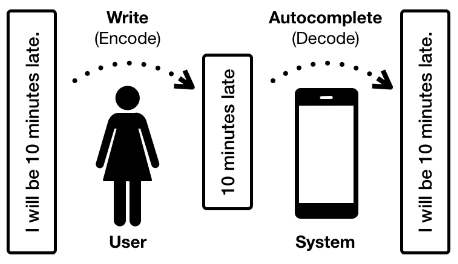
\includegraphics[width=.5\linewidth]{figs/autocomplete_game.png}
    \caption{schematic overview of the communication game. Figure from \protect\citeA{autocomplete}.}
    \label{fig:autocomplete}
\end{figure}

The same autocomplete communication game is considered as in \citeA{autocomplete}. In this game, a human (called user) encodes a sentence into keywords. 
These keywords are then decoded by a machine (called system) to retrieve the full, initial sentence. 
A schematic overview is given in figure \ref{fig:autocomplete}. 
The communication game is succesfull if the retrieved sentence is the same as the initial sentence. 

More formally, a target sentence $x=(x_1, \dots, x_m)$ is communicated by a user through the keywords $z=(z_1, \dots, z_n)$. 
Note that $z$ is a subsequence of $x$. 
The system then tries to retrieve the target sentence by decoding the keywords. 
The target sentence is described by the keywords using encoding strategy $q_{\alpha}(z | x)$ and the system decodes the keywords by using decoding strategy $p_{\beta}(x|z)$. 

For a model to be efficient, the number of keywords needs to be as low as possible. 
In addition, for a model to be accurate, the probability of reconstructing $x$ from $z$ needs to be as high as possible. 
Therefore, a cost and a loss, respectively, can be defined:
\begin{equation}
    \label{eq:cost}
    \text{cost}(x,\alpha) = \mathbb{E}_{q_{\alpha}(z|x)} [\text{length}(z)]
\end{equation}
\begin{equation}
    \label{eq:loss}
    \text{loss}(x,\alpha,\beta) = \mathbb{E}_{q_{\alpha}(z|x)} [-\log p_{\beta}(x|z)]
\end{equation}

\subsection{Segmentation model}
% Why does a segmentation model work?
% TODO: better captions for images
% TODO: add references
% TODO: add Markov Models

\paragraph{General idea.}
\textcolor{orange}{With a segmentation model all possible segmentation can be made. 
A segmentation model scores every possible segmentation.
With these scores, the model can determine what the best possible segmentation is.}

\paragraph{Segmentation model for text.}
So how does the segmentation model work for text? 
If we have a sentence, e.g. \textit{'I will be late'}, we can use fencepost indexing and represent the fenceposts as nodes in a directed acyclic graph (DAG). 
We can then draw edges between those nodes that represent segments. 
Those segments can be seen as (groups of) words. 
In figure \ref{fig:dag}, a DAG can be seen in which all the possible segments are showed. 
In the case of the autocomplete communication model described before, a segment is either kept or not.
Therefore, we can have one edge representing 'keep' and one representing 'do not keep', resulting in figure \ref{fig:dag2}.
If the pink edges are taken as 'do not keep' and the blue ones as 'keep', two possible segmentations can be seen in figure \ref{fig:segmentation} and \ref{fig:segmentation2}. 
Both segmentations result in the keywords \textit{'will be late'}. 

\begin{figure}
    \centering
    \begin{subfigure}[b]{0.45\textwidth}
        \centering
        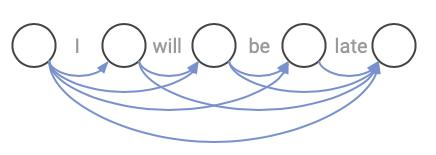
\includegraphics[width=\textwidth]{figs/segmentation1.jpeg}
        \caption{Segments as a DAG}
        \label{fig:dag}
    \end{subfigure}
    \hfill
    \begin{subfigure}[b]{0.45\textwidth}
        \centering
        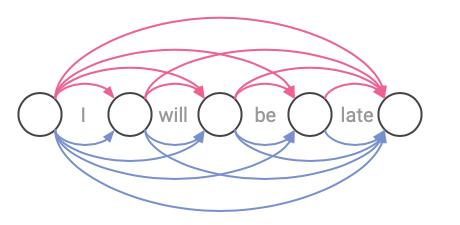
\includegraphics[width=\textwidth]{figs/segmentation2.jpeg}
        \caption{More segments as a DAG}
        \label{fig:dag2}
    \end{subfigure}
    \hfill
    \begin{subfigure}[b]{0.45\textwidth}
        \centering
        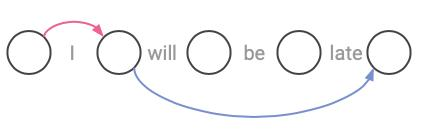
\includegraphics[width=\textwidth]{figs/segmentation3.jpeg}
        \caption{Possible segmentation}
        \label{fig:segmentation}
    \end{subfigure}
    \hfill
    \begin{subfigure}[b]{0.45\textwidth}
        \centering
        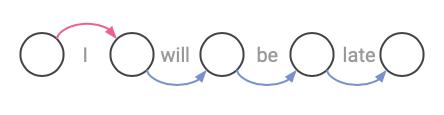
\includegraphics[width=\textwidth]{figs/segmentation4.jpeg}
        \caption{Another possible segmentation}
        \label{fig:segmentation2}
    \end{subfigure}
    \caption{Segmentation model.}
    \label{fig:segmentation_model}
\end{figure}

The best segmentations can be found with the help of dynamic programming algorithms such the Viterbi and the forward algorithms. 
% TODO: add HMMs

\subsection{Structured latent variables}
A latent variable is an unobservable variable.
For these variables, there are no labels available. 
Therefore, it is not possible to use supervised learning on them. 
In the case of this model, we try to recover the full sentence by inferring what is a good mask.
The mask determines what words are good keywords and thus is a latent variable. 
In addition, the segmentation model makes this a structured variable. 


\section{Current research}
% Gap
% Research question: To what extend can a segmentation model help by selecting keywords for an auto-complete communication game?
% TODO: check references - are they relevant?

Previous research did not take structure into account \cite{autocomplete, Bar-YossefZiv2011Cqa, SvyatkovskiyAlexey2019PACC}.
Since language is structured, it makes sense to use a structured model as an autocomplete model. 
In this research, we look at how we can use a latent segmentation model to retrieve keywords from a sentence. 
The segmentation model will be implemented in the encoder of the encoder-decoder model in order to choose the best keywords from the sentence.

\chapter{Experiment 1 \\ Replication}
\label{ch:repl}
In the first experiment the autoencoder model from \citeA{autocomplete} was replicated. 

\section{Method}
To replicate the model, an encoder-decoder model was made. The encoder chooses which words to keep as keywords, and the decoder tries to retrieve the full sentence of the keywords. 

\subsection{Data}
\label{sec:data}
% TODO: make a table with a few example sentences
% TODO: descirbe train, validation and test set
The same data was used as in \citeA{autocomplete}.
The data used to train the model consisted of 500K randomly sampled sentences from the Yelp restaurant reviews corpus \cite{data}.
Another 50K sentences were used to test the model. 
The sentences had at most 16 tokens. 
The reviews were segmented into sentences following the same procedure as in \citeA{GuuKelvin2018GSbE}. 

The model of \citeA{autocomplete} also predicts capital letters and whitespaces. 
However, for English we can just assume that after every word a space is used. 
Therefore, the data was adjusted to leave out the characters for whitespaces. 
Something similar is also true for capital letters: usually these only occur at the start of a sentence or in names. 
It is thus not necessary to also predict capital letters. 

\noindent\textcolor{red}{TODO: \begin{enumerate}
    \item Table with example sentences
    \item Adjust the number of sentences used for the training and the test set
\end{enumerate}}

\subsection{Experimental Design}
The model used is an encoder-decoder model.
The encoder, using the encoding strategy $q_{\alpha}(z|x)$, takes as input a target sequence $x = (x_1, \dots, x_m)$ and outputs a sequence of keywords $z = (z_1, \dots, z_n)$.
The decoder, using the decoding strategy $p_{\beta}(x|z)$, then takes these keywords as input and outputs a predicted sequence $y = (y_1, \dots, y_k)$. 
The better the autoencoder works, the more likely it is that $x$ and $y$ are equal. 

\subsection{Model description}
\label{sec:model}
% TODO: add diagram?
\paragraph{Encoder.} 
The encoder embeds the tokens and uses a uni-directional LSTM to score the tokens.
An additional linear layer followed by sigmoid function is used to determine the probability of keeping each token. 
From these probabilities, a mask is sampled from a Bernoulli distribution. 
Finally, the sequence of kept tokens and the log probability of the mask are returned.

\paragraph{Decoder.} 
The decoder itself is also an encoder-decoder model (the encoder of this model is referred to as encoder*).
The encoder* first embeds the tokens of the subsequence.
It then encodes the embedding using a bi-directional LSTM. 

The decoder decodes the full sentence. 
It therefore embeds the already decoded sequence (or just the <sos> symbol if there is none) into a 300-dimensional vector and concatenates the last hidden state of the encoder* to it. 
This embedding is the input for another uni-directional LSTM. 
Finally, the probability of the next word is calculated using global attention and the full sentence and its log probability are returned. 

During training, the decoder is given the keywords and at every step the model takes the correct word from the target sequence and calculates the probability of that sequence.
During testing, however, the decoder uses a greedy decoding strategy and thus takes the word with the highest probability as the next word. 
% TODO: <sos> anders verwoorden

\paragraph{Optimization.} 
The goal of the model is to be as efficient and accurate as possible. 
If equation \ref{eq:cost} and \ref{eq:loss} are merged and a parameter $\lambda$ is added to represent the trade-off between the two, the goal becomes the following:
\begin{equation}
    \label{eq:loss2}
    \min_{\alpha, \beta} \mathbb{E} [\text{cost}(x, \alpha)] + \lambda \cdot \mathbb{E}[\text{loss}(x, \alpha, \beta)].
\end{equation}
Here the expactation is taken over $x$. 
Since the gradients of equation \ref{eq:loss2} cannot be calculated, it is approximated with Monte Carlo.
The gradients can then by calculated as following (see appendix \ref{app:gradients} for the exact derivations):

\begin{equation}
    \label{eq:gradient_alpha}
    \nabla_\alpha F(x, z, \alpha, \beta) = \mathbb{E}_{q_{\alpha}(z|x)} [\nabla_{\alpha} \log q_{\alpha}(z|x) f(x, z, \beta)],
\end{equation}
\begin{equation}
    \label{eq:gradient_beta}
    \nabla_\beta F(x, z, \alpha, \beta) = \mathbb{E}_{q_{\alpha}(z|x)} [\nabla_{\beta} f (x, z, \beta)].
\end{equation}
Where, $f$ and the score function estimator (SFE) $F$ (and its Monte Carlo approximation) are:
\begin{equation}
    \label{eq:f}
    f(x, z, \beta) = \text{length}(z) + \lambda \cdot (-\log p_{\beta}(x|z)),
\end{equation}
\begin{equation}
    \label{eq:F}
    F (\alpha, \beta) = \mathbb{E}_{q_{\alpha}(z|x)} [f(x, z, \beta)],
\end{equation}
\begin{equation}
    \label{eq:F_approx}
    F (\alpha, \beta) \approxtext{M.C.} \frac{1}{M} \sum_i f (x, z^{(i)}, \beta).
\end{equation}
Here $M$ is the amount of samples drawn from $q_{\alpha}(z|x)$.

\subsection{Hyperparameters}
\label{sec:hyper}
During training, the sentences start with a <sos> symbol and end with a <eos> symbol.
During testing of the model, those symbols are removed.

The model is implemented using PyTorch \cite{pytorch}.
After each token is embedded, ReLu is used. During training, dropout is used to prevent overfitting. 
The hidden dimensions of the LSTM layers are all 300. 
To optimize the model an Adam optimizer is used with a learning rate of 0.01. 
The model was trained for 30 epochs.

\subsection{Optimizations}
To let the model predict better results faster, a few optimizations were done.
\paragraph{Copy mechanism.} The copy mechanism in the decoder determines if it wants to copy the current token or wants to generate a new token. 
It therefore calculates the probability of the new word as following:
\begin{equation}
    p(w) = (1 - p_{\text{gen}}) \cdot p_{\text{copy}}(w) + p_{\text{gen}} \cdot p_{\text{word}}(w).
\end{equation}
For the calculation of the probability of the to be copied word, $p_{\text{copy}}(w)$, the global attention mechanism from the decoder is used. 
To calculate the probability of generating a new word, $p_{\text{gen}}$, the last hidden decoder state, the attention mechanism and the token embedding of the new to generated word are used in a linear layer followed by a sigmoid.
$p_{\text{word}}(w)$ is the probability of the to be generated word if a word is being generated. 

\paragraph{Adjusted datasets.} The train and test set were adjusted so that the test set is a subset of the training set. 
A reason for this was the many unkown tokens in the test set if this was not done. 
\citeA{autocomplete} used the copy mechanism and a dynamic vocabulary for this, but for the task at hand and the amount of data this also works.

\paragraph{Variance reduction.} Because of the use of a SFE the gradient can be more prone to noise \cite{niculae2023discretelatentstructureneural}.
To solve this problem, its variance can be reduced in a couple of ways. 
One of those solutions is to sample a second subsentence in the encoder. 
With this second subsentence, $f(z')$ can be determined and the loss can be updated as following:
\begin{equation}
    \mathbb{E}_{q_{\alpha}(z|x)} [\nabla_w \log q_{\alpha}(z|x) \cdot (f(z)-f(z'))] + \mathbb{E}_{q_{\alpha}(z|x)} [\nabla_w f(z)]
\end{equation}
Where $w$ is a parameter. Note that the gradient is not changed when subtracting $f(z')$ from $f(z)$ since it is a constant which is independent of $w$.


\section{Results}

\chapter{Experiment 2 \\ Segmentation Model}
In the second experiment, the model from chapter \ref{ch:repl} is expanded with a segmentation model. 

\section{Method}
Another autoencoder model is made in which the encoder uses a segmentation model to choose the sequence of keywords $z$.
The same data was used as described in section \ref{sec:data}.

\subsection{Score matrix}
In order for this model to work, it needs a score tensor, $a$.
This tensor consists of two upper triangle matrices of $m+1 \times m+1$.
Both matrices represent the score of the segments, one for the segment when it is true, and one for when the segment is false.
% TODO: How is the tensor constructed?

\subsection{Model description}
The same model as in section \ref{sec:model} was used. 
Only the encoder part was adjusted.
Instead of using an LSTM and a linear layer to score each token, the segmentation model is used.
% TODO: What does the segmentation model look like exactly?

\subsection{Hyperparameters}
The same hyperparameters as in section \ref{sec:hyper} were used.
In addition, for the segmentation model ...
% TODO: describe parameters of the segmentation model

\subsection{(Optimizations)}
% (TODO: describe optimizations done for the segmentation model)

\section{Results}

\chapter{Results}

\chapter{Conclusion}

\chapter{Discussion}

\bibliography{articles.bib}
\bibliographystyle{apacite}

\appendix
\chapter{Optimization derivations}
\label{app:gradients}
Using equations \ref{eq:cost} and \ref{eq:loss}, the goal is:
\begin{align*}
    \quad & \min_{\alpha, \beta} \mathbb{E} [\text{cost}(x, \alpha)] + \lambda \cdot \mathbb{E}[\text{loss}(x, \alpha, \beta)] \\
    &= \min_{\alpha, \beta} \mathbb{E} [\text{cost}(x, \alpha) + \lambda \cdot \text{loss}(x, \alpha, \beta)] \\
    &= \min_{\alpha, \beta} \frac{1}{D} \sum_{x \in D}[\text{cost}(x, \alpha) + \lambda \cdot \text{loss}(x, \alpha, \beta)].
\end{align*}
Here $D$ is the set of all target sentences. \\

\noindent Then $f$ can be defined as:
\begin{align*}
    f(x, z, \beta) = \text{length}(z) + \lambda \cdot (-\log p_{\beta}(x|z)).
\end{align*}

\noindent And $F$ as:
\begin{align*}
    F(x, z, \alpha, \beta) &= \mathbb{E}_{q_{\alpha}(z|x)} [[\text{length}(z) + \lambda \cdot (-\log p_{\beta}(x|z))]] \\
    &=^{\ast} \sum_{z\in Z} [q_{\alpha}(z|x) f(x, z, \beta)] \\
    &= \mathbb{E}_{q_{\alpha}(z|x)}[f(x, z, \beta)],
\end{align*}
where $Z$ consists of all the possible masks of size $x$.
In the step marked with *, the law of the unconscious statistician is used: $\mathbb{E}_{P(A)}[f(A)] = \sum_{a \in A}P(a)f(a)$. \\

\noindent Thus, the goal then becomes:
\begin{align*}
    \min_{\alpha, \beta} F(x, z, \alpha, \beta).
\end{align*}

\noindent The gradient with respect to $\alpha$ can be calculated as following:
\begin{align*}
    \nabla_{\alpha} F(x, z, \alpha, \beta) &= \nabla_{\alpha} \mathbb{E}_{q_{\alpha}(z|x)} [f(x, z, \beta)] \\
    &= \nabla_{\alpha} \sum_z [q_{\alpha}(z|x) f(x, z, \beta)] \\
    &= \sum_z \nabla_{\alpha} (q_{\alpha}(z|x) f(x, z, \beta)) \\
    &=^\ast \sum_z (q_{\alpha}(z|x) [\nabla_{\alpha} \log q_{\alpha}(z|x) f(x, z, \beta)]) \\
    &= \mathbb{E}_{q_{\alpha}(z|x)} [\nabla_{\alpha} \log q_{\alpha}(z|x) f(x, z, \beta)].
\end{align*}
In the step marked with *, a log-derivative trick is used: $\nabla_t \log h(t) = \frac{\nabla_t h(t)}{h(t)}$. \\

\noindent And the gradient with respect to $\beta$:
\begin{align*}
    \nabla_{\beta} F(x, z, \alpha, \beta) &= \nabla_{\beta} \mathbb{E}_{q_{\alpha}(z|x)}[f(x, z, \beta)] \\
    &= \nabla_{\beta} \sum_z [q_{\alpha}(z|x)f(x, z, \beta)] \\
    &= \sum_z \nabla_{\beta} (q_{\alpha}(z|x)f(x, z, \beta)) \\
    &= \sum_z (q_{\alpha}(z|x) [\nabla_{\beta} f(x, z, \beta)]) \\
    &= \mathbb{E}_{q_{\alpha}(z|x)} [\nabla_{\beta} f(x, z, \beta)].
\end{align*}

\end{document}